\section{Výsledná aplikace}

Následující obrázky ukazují jednotlivé části a funkce výsledné aplikace, která slouží k tvorbě digitálního modelu terénu pomocí Delaunay triangulace, generování vrstevnic, výpočtu sklonu a expozice a základní 3D vizualizaci. Aplikace umožňuje načíst vlastní data nebo generovat syntetické tvary terénu.

\begin{figure}[H]
    \centering
    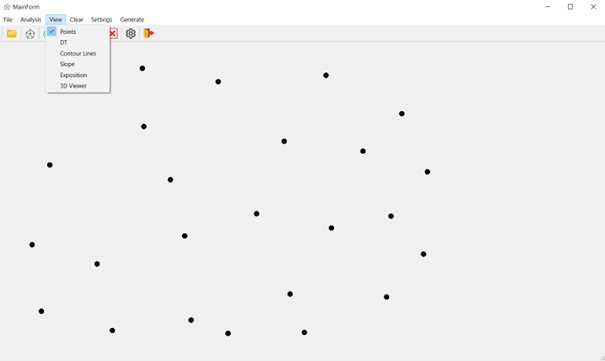
\includegraphics[width=\textwidth]{images/Ukazka_aplikace.png}
    \caption{Hlavní okno aplikace s ovládacími prvky}
\end{figure}

\begin{figure}[H]
    \centering
    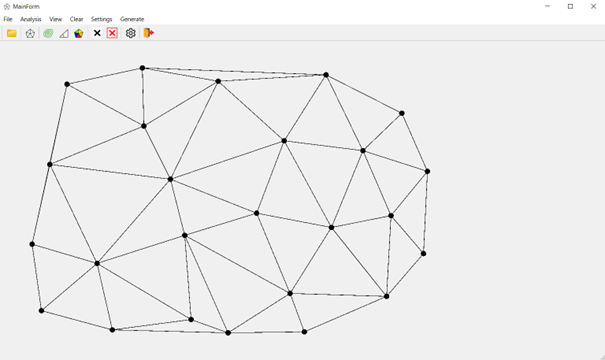
\includegraphics[width=\textwidth]{images/Ukazka_DT.png}
    \caption{Vytvořená Delaunay triangulace (TIN) ze zadaných bodů}
\end{figure}

\begin{figure}[H]
    \centering
    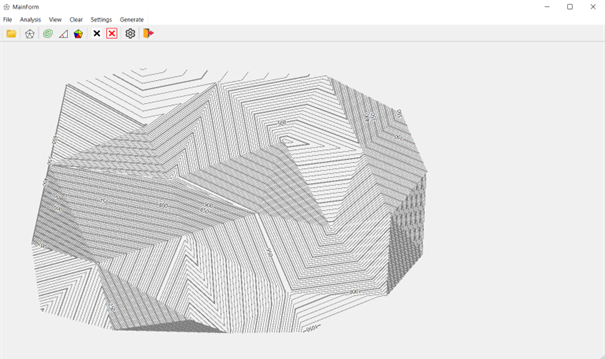
\includegraphics[width=\textwidth]{images/Ukazka_contourlines.png}
    \caption{Vizualizace vrstevnic vytvořených lineární interpolací}
\end{figure}

\begin{figure}[H]
    \centering
    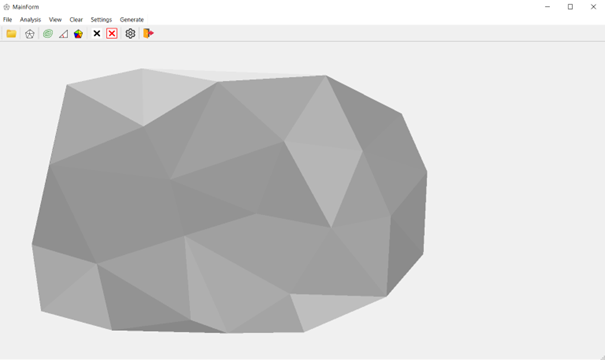
\includegraphics[width=\textwidth]{images/Ukazka_slope.png}
    \caption{Barevná vizualizace sklonu (slope) jednotlivých trojúhelníků}
\end{figure}

\begin{figure}[H]
    \centering
    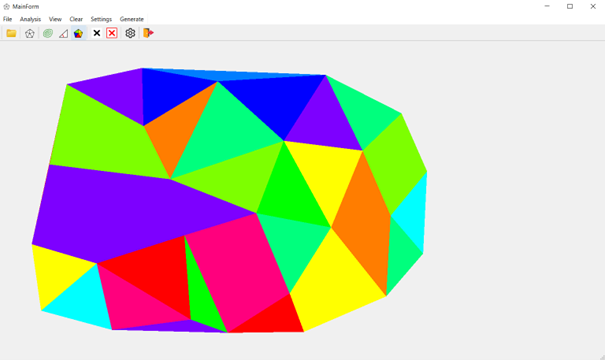
\includegraphics[width=\textwidth]{images/Ukazka_aspect.png}
    \caption{Barevná vizualizace expozice (aspekt) jednotlivých trojúhelníků}
\end{figure}

\begin{figure}[H]
    \centering
    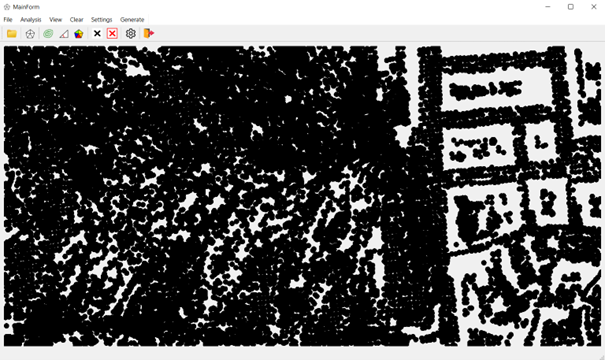
\includegraphics[width=\textwidth]{images/Ukazka_petrin_body.png}
    \caption{Načtení reálných dat – okolí Petřína (data z DMR 5G)}
\end{figure}

\begin{figure}[H]
    \centering
    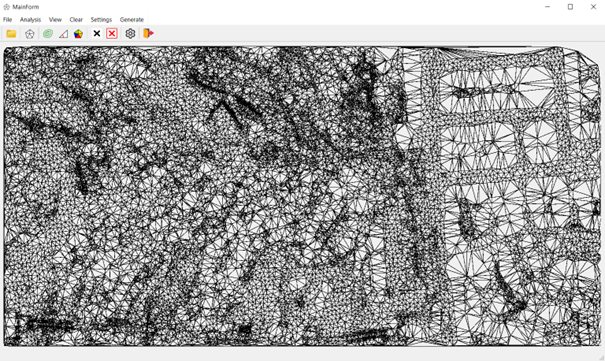
\includegraphics[width=\textwidth]{images/Ukazka_petrin_DT.png}
    \caption{Delaunayova triangulace – okolí Petřína (data z DMR 5G)}
\end{figure}

\begin{figure}[H]
    \centering
    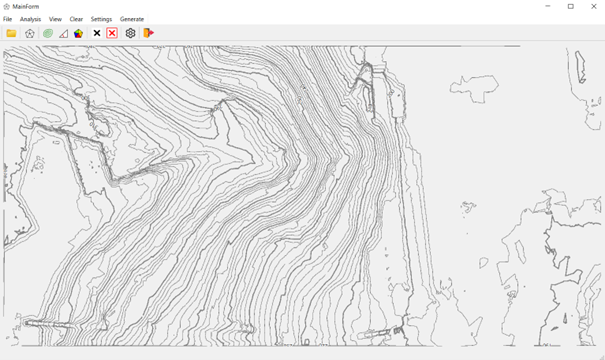
\includegraphics[width=\textwidth]{images/Ukazka_petrin_contourlines.png}
    \caption{Vrstevnice – okolí Petřína (data z DMR 5G)}
\end{figure}

\begin{figure}[H]
    \centering
    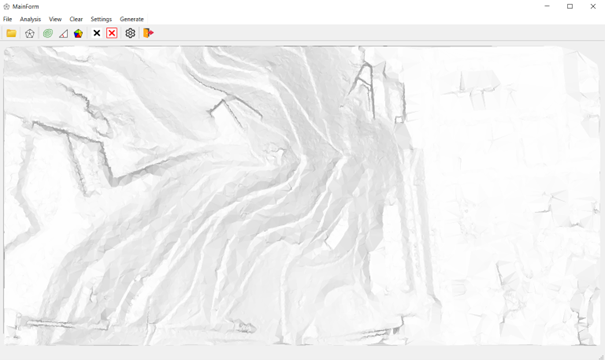
\includegraphics[width=\textwidth]{images/Ukazka_petrin_slope.png}
    \caption{Sklon (slope) – okolí Petřína (data z DMR 5G)}
\end{figure}

\begin{figure}[H]
    \centering
    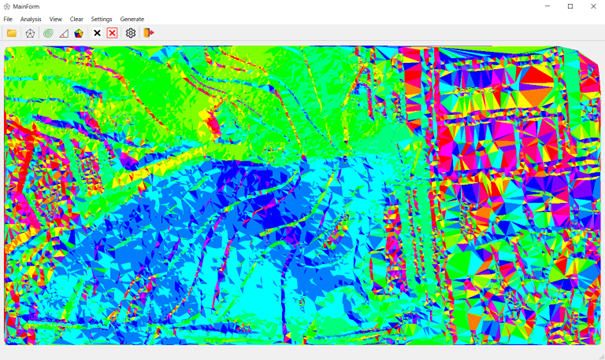
\includegraphics[width=\textwidth]{images/Ukazka_petrin_aspect.png}
    \caption{Expozice (aspect) – okolí Petřína (data z DMR 5G)}
\end{figure}

\begin{figure}[H]
    \centering
    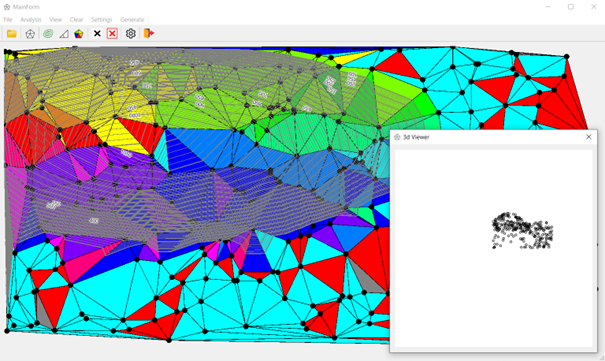
\includegraphics[width=\textwidth]{images/ukazka_kopec.png}
    \caption{Ukázka uměle vygenerované kupy}
\end{figure}

\begin{figure}[H]
    \centering
    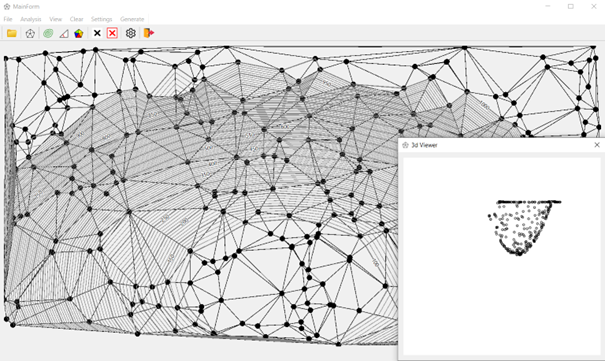
\includegraphics[width=\textwidth]{images/ukazka_udoli.png}
    \caption{Ukázka uměle vygenerovaného údolí}
\end{figure}

\begin{figure}[H]
    \centering
    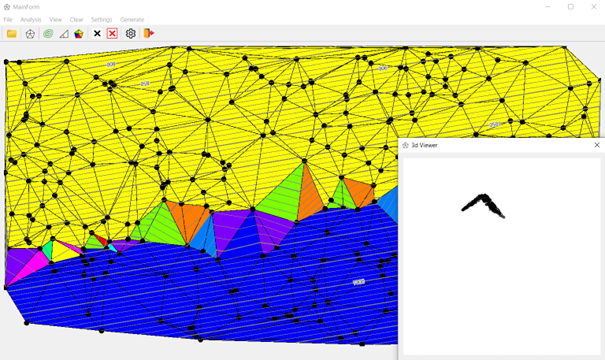
\includegraphics[width=\textwidth]{images/ukazka_hrbet.png}
    \caption{Ukázka uměle vygenerovaného hřbetu}
\end{figure}

\begin{figure}[H]
    \centering
    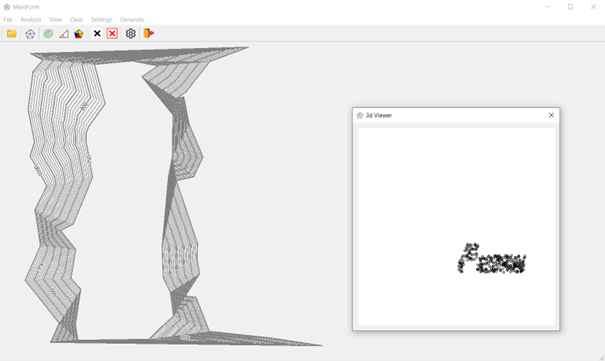
\includegraphics[width=\textwidth]{images/ukazka_spocinek.png}
    \caption{Ukázka uměle vygenerovaného spočinku}
\end{figure}

\begin{figure}[H]
    \centering
    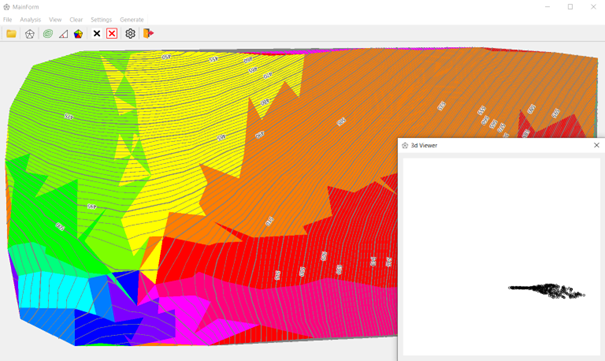
\includegraphics[width=\textwidth]{images/ukazka_sedlo.png}
    \caption{Ukázka uměle vygenerovaného sedla}
\end{figure}
